\documentclass{beamer}

\newcommand{\delim}{\line(1,0){290}}
\newcommand{\norma}[1]{\Vert #1 \Vert_2}
\newcommand{\prodint}[2]{\langle #1,#2 \rangle}

\colorlet{teal}[rgb]{blue!50!green}
%\setbeamercolor{cordotitulo}{bg=green!30!black,fg=white}
\useinnertheme{rounded}
\setbeamercolor{structure}{fg=teal!80!blue}
%\useoutertheme{smoothbars}
%\useoutertheme{shadow}
\useoutertheme[height=1 cm,width=1.5 cm]{sidebar}
%\usecolortheme{crane}
%\setbeamerfont{frametitle}{shape=\itshape}
\setbeamercolor{palette primary}{bg=teal!80!blue,fg=white}
\setbeamercolor{palette secondary}{bg=white,fg=white} %cor do logo
\setbeamercolor{palette tertiary}{bg=blue!70!black,fg=white}
\setbeamercolor{palette quaternary}{bg=white,fg=teal!80!blue}
\setbeamercolor{sidebar}{bg=teal!80!blue}
%\setbeamercolor{palette sidebar primary}{bg=red,fg=black}
%\setbeamercolor{palette sidebar secondary}{bg=red,fg=black}
\setbeamercolor{palette sidebar tertiary}{fg=white} %Autor no sidebar
\setbeamercolor{palette sidebar quaternary}{fg=white} %Titulo no sidebar
\setbeamercolor{section in sidebar}{fg=teal!80!blue,bg=white} %A cor naum
\setbeamercolor{subsection in sidebar}{fg=teal!80!blue,bg=white} %A cor naum
%ativa parece ser uma media das duas
%\setbeamercolor{section in sidebar current}{fg=red}
\setbeamercolor{frametitle}{fg=white,bg=teal!80!blue} %mudar
%fg aqui
\setbeamercolor{title}{bg=teal!80!blue,fg=white}
\setbeamerfont{title}{series=\bf}
\setbeamercolor{author}{bg=teal!80!blue,fg=white}
\setbeamerfont{author}{series=\bf}
\setbeamercolor{normal text}{bg=white,fg=teal!50!black}
\logo{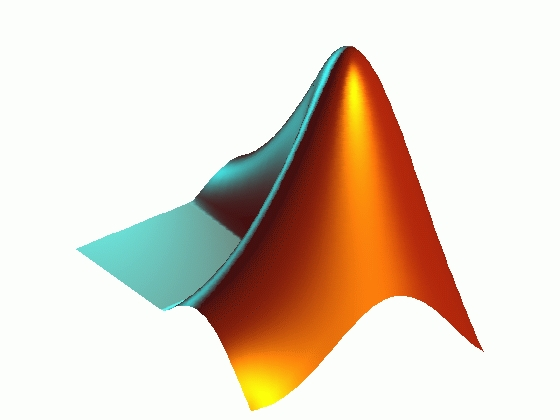
\includegraphics[scale=0.06]{matlab_logo.jpg}}

\title{Introdu\c{c}\~ao ao MatLab \\ Aula 3}
\author{Abel Siqueira \\ Kally Chung}
\date{}

\begin{document}

\frame{\titlepage}

\section[Fun\c{c}\~oes]{}
\begin{frame}[fragile]

  \frametitle{Fun\c{c}\~oes}
  
  \begin{itemize}
  \item<1-> O Matlab tem uma quantidade imensa de fun\c{c}\~oes prontas.
  \item<2-> Para usar as fun\c{c}\~oes basta escrever o nome delas na janela de comando do Matlab junto com os argumentos, se ouver.
  \item<3-> Tamb\'em \'e poss\'ivel criar fun\c{c}\~oes no Matlab, para depois poder cham\'a-las.
  \item<4-> Fun\c{c}\~oes tamb\'em s\~ao chamadas de rotinas.
  \item<5-> \'E poss\'ivel descobrir para que serve uma fun\c{c}\~ao usando o comando {\tt help}.
  \end{itemize}

\end{frame}

\begin{frame}[fragile]
\frametitle{Fun\c{c}\~oes Matem\'aticas}
Algumas fun\c{c}\~oes matem\'aticas que passamos na aula 1 funcionam apenas em n\'umeros, outras tamb\'em funcionam em vetores e matrizes. Veja:
{\scriptsize
\begin{verbatim}
>> v = [-1 0 1];
>> exp(v)
ans =
    0.3679    1.0000    2.7183
>> abs(v)
ans =
     1     0     1
\end{verbatim}
}

\end{frame}

\subsection[Arquivos m]{}

\begin{frame}
\frametitle{Arquivos m}

Para criarmos nossas pr\'oprias fun\c{c}\~oes no Matlab, utilizaremos o editor de arquivos m do Matlab. Veja como abri-lo:
\begin{center}
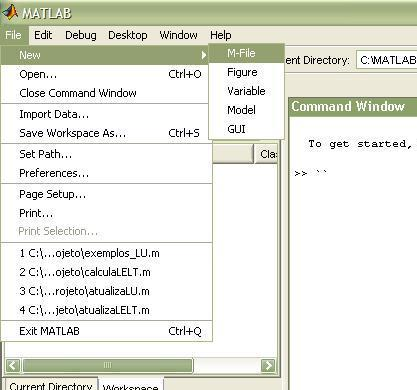
\includegraphics[scale=0.5]{figura4.jpg}
\end{center}

\end{frame}

\begin{frame}
 \frametitle{Editor}

 O editor de arquivos m do Matlab parece um editor normal:
 \begin{center}
 \includegraphics[scale=0.4,border=1]{figura5.jpg}
 \end{center}

\end{frame}

\begin{frame}
 \frametitle{Sintaxe}

A sintaxe para qualquer fun\c{c}\~ao que quisermos criar \'e:

{\scriptsize \tt function [<variaveis\_saida] = <nome\_da\_funcao>(<variaveis\_entrada>)}

\begin{itemize}
\item<2-> Se existir apenas uma vari\'avel de sa\'ida, n\~ao \'e necess\'ario utilizar os colchetes.
\item<3-> Se n\~ao existirem vari\'aveis de entrada, n\~ao \'e necess\'ario o par\^enteses.
\item<4-> Se n\~ao existirem nem vari\'aveis de entrada, $\times \times \times$
\end{itemize}

\end{frame}

\begin{frame}[fragile]
 \frametitle{Primeira Fun\c{c}\~ao}

Vamos criar uma fun\c{c}\~ao que recebe dois elementos e os soma:

\begin{itemize}
 \item<1-> Abra o editor.
 \item<2-> Escreva {\tt function s = soma(a,b)}.
 \item<3-> Na linha seguinte, atribua \`a vari\'avel s, a soma dos elementos a e b.
 \item<4-> Salve o documento {\bf com o mesmo nome da fun\c{c}\~ao}, neste caso, soma. Note que a extens\~ao desse arquivo \'e .m.
\end{itemize}
\pause \pause \pause \pause
Seu arquivo deve ter ficado assim:
\delim
\begin{verbatim}
function s = soma(a,b)

s = a + b;
\end{verbatim}

\end{frame}

\begin{frame}[fragile]
\frametitle{Primeira Fun\c{c}\~ao}
Volta para a janela de comando do matlab e chame a sua fun\c{c}\~ao.
\pause
{\scriptsize
\begin{verbatim}
>> soma(3,4)
ans =
     7
>> s = soma(3,4);
>> s
s =
     7
\end{verbatim}}
\pause
Note que, se voc\^e esqueceu o ; depois de {\tt s = a + b}, ent\~ao acontecer\'a o seguinte:
\pause
{\scriptsize
\begin{verbatim}
>> soma(3,4)
s =
     7
ans =
     7
\end{verbatim}}

\end{frame}

\begin{frame}

\frametitle{Segunda Fun\c{c}\~ao}

Agora vamos criar uma nova fun\c{c}\~ao. Esta deve receber dois vetores, $v$ e $w$ e calcular o \^angulo $\theta$ entre eles, e a proje\c{c}\~ao de $v$ sobre $w$.
\pause

Como calcula o \^angulo?
\pause

Lembre-se que
$$\prodint{v}{w} = \norma{v}\norma{w}\cos(\theta)$$
\pause

Ent\~ao
$$\theta = \arccos\bigg(\frac{\prodint{v}{w}}{\norma{v}\norma{w}}\bigg)$$

\end{frame}

\begin{frame}
\frametitle{Segunda Fun\c{c}\~ao}

E como calcula a proje\c{c}\~ao?
\pause

$$\mbox{proj}_wv = \frac{\prodint{v}{w}}{\norma{w}^2}w$$
\pause

Lembre-se que os comandos utilizados aqui s\~ao:

\begin{itemize}
\item Produto Interno $\prodint{v}{w}$: {\tt dot(v,w)}
\item Norma $\norma{v}$: {\tt norm(v)}
\item $\arccos{x}$: {\tt acos(x)}
\end{itemize}
\pause
Fa\c{c}am!

\end{frame}

\begin{frame}[fragile]
\frametitle{Segunda Fun\c{c}\~ao}

Uma das maneiras de escrever essa fun\c{c}\~ao \'e:

{\scriptsize
\begin{verbatim}
function [theta,proj] = aula3(v,w)

theta = acos(dot(v,w)/(norm(v)*norm(w)));
proj = (dot(v,w)/norm(w)^2)*w;
\end{verbatim}
}

\pause
Note, no entanto que calculamos {\tt dot(v,w)} e {\tt norm(w)} duas vezes, ou seja, fazemos a mesma conta duas vezes. Podemos resolver isso fazendo
\pause

{\scriptsize
\begin{verbatim}
function [theta,proj] = aula3(v,w)

prodint = dot(v,w);
Nw = norm(w);
Nv = norm(v);

theta = acos(prodint/(Nw*Nv));
proj = (prodint/Nw^2)*w;
\end{verbatim}
}

\end{frame}

\begin{frame}
\frametitle{Arquivos M}

\begin{itemize}
 \item<1-> Quando gravamos um arquivo M e queremos us\'a-lo, este arquivo deve estar no Diret\'orio Atual do Matlab.
 \item<2-> Muitos dos ``Erros'' que achamos que est\'a acontecendo com o Matlab, na verdade acontecem porque n\~ao estamos no diret\'orio correto.
\end{itemize}
\end{frame}

\subsection[Usando o Help]{}

\begin{frame}
\frametitle{Usando o {\tt help}}

\begin{itemize}
\item<1-> Para descobrir para que serve algum comando no Matlab, basta digitas {\tt help <comando>}.
\item<2-> O Matlab exibe n\~ao s\'o para que serve o comando, mas tamb\'em quais os poss\'iveis argumentos para ele, e algumas vezes um exemplo.
\item<3-> Digitando {\tt help} sem nenhum comando a mais, o Matlab exibe uma lista de t\'opicos onde pode-se pesquisar sobre como funciona o Matlab e suas ferramentas.
\item<4-> \'E um bom recurso para quando n\~ao lembramos como usar o comando, mas sabemos que o comando existe.
\end{itemize}

\end{frame}

\begin{frame}[fragile]
\frametitle{Usando o {\tt help}}

Veja por exemplo, um peda\c{c}o do help do comando {\tt exp}:
\pause

\begin{verbatim}
>> help exp
Ah, vai dizer que naum sabe usar o exp
\end{verbatim}

\end{frame}


\section[Exerc\'icios]{}

\begin{frame}
\frametitle{Exerc\'icios}

\begin{enumerate}
\item Escreva um programa que recebe dois n\'umeros e retorna o maior e o menor deles, sem usar as fun\c{c}\~oes {\tt max} e {\tt min}. (Dica: Use a fun\c{c}\~ao {\tt abs}).
\item Escreva um programa que receba uma matriz $A$, um vetor $x$. Seu programa deve retornar o vetor $Ax$ e o escalar $x^TAx$.
\item Descubra para que serve o comando {\tt triu}.
\end{enumerate}

\end{frame}


\end{document}